%!TEX root = main.tex
\section{Supplementary Simulation Results}
\label{sec:simsupplement}
This section discusses additional simulation results for the choosing instrumental variables example, as a supplement to those given in Section \ref{sec:chooseIVsim}.

\subsection{Downward J-Test}
\label{sec:downwardJ}
The downward $J$-test is an informal but fairly common procedure for moment selection in practice.
In the context of the simulation example from Section \ref{sec:chooseIVsim} it amounts to simply using the full estimator unless it is rejected by a $J$-test.
Table \ref{fig:chooseIVsim_RMSErelJ} compares the RMSE of the post-FMSC estimator to that of the downward $J$-test with $\alpha = 0.1$ (J90), and $\alpha = 0.05$ (J95).
For robustness, I calculate the $J$-test statistic using a centered covariance matrix estimator, as in the FMSC formulas from section \ref{sec:chooseIVexample}.
Unlike the FMSC, the downward $J$-test is very badly behaved for small sample sizes, particularly for the smaller values of $\gamma$.
For larger sample sizes, the relative performance of the FMSC and the $J$-test is quite similar to what we saw in Figure \ref{fig:OLSvsIV_RMSEbaseline} for the OLS versus TSLS example: the $J$-test performs best for the smallest values of $\rho$, the FMSC performs best for moderate values, and the two procedures perform similarly for large values.
\begin{figure}
\centering
	% Created by tikzDevice version 0.7.0 on 2014-07-01 17:48:04
% !TEX encoding = UTF-8 Unicode
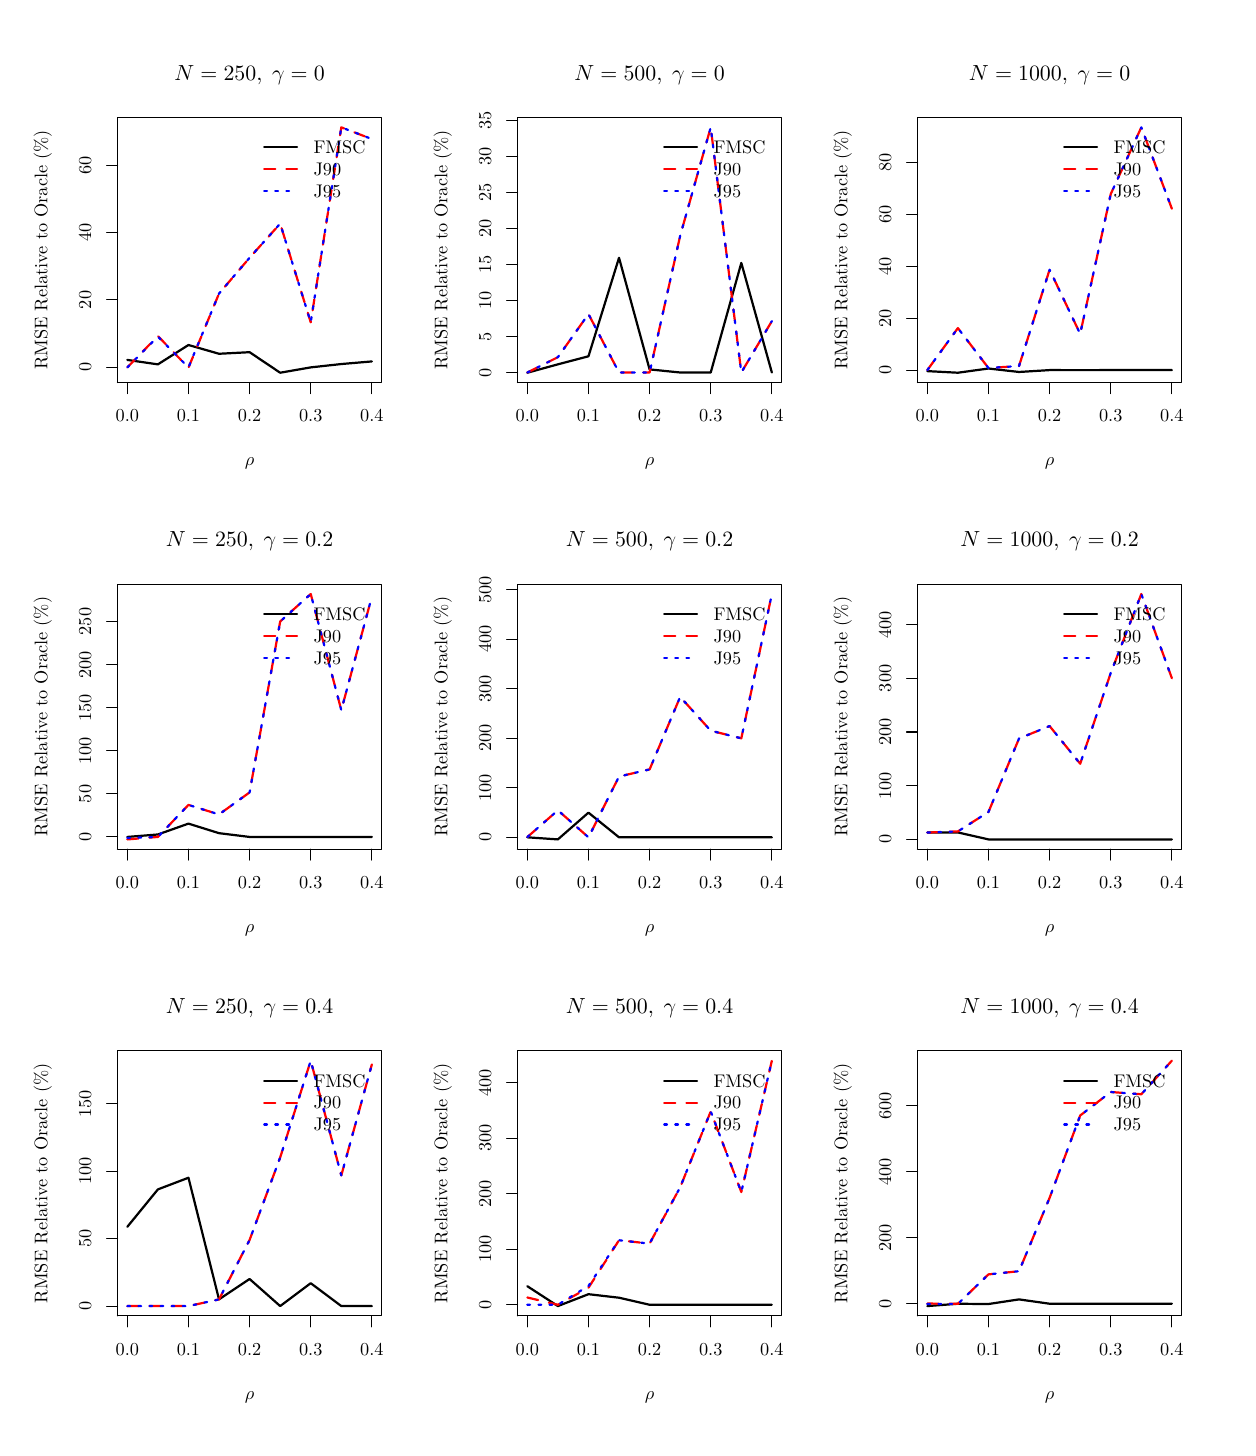
\begin{tikzpicture}[x=1pt,y=1pt]
\definecolor[named]{fillColor}{rgb}{1.00,1.00,1.00}
\path[use as bounding box,fill=fillColor,fill opacity=0.00] (0,0) rectangle (433.62,505.89);
\begin{scope}
\path[clip] ( 32.47,377.65) rectangle (127.91,473.42);
\definecolor[named]{drawColor}{rgb}{0.00,0.00,0.00}

\path[draw=drawColor,line width= 0.8pt,line join=round,line cap=round] ( 36.01,385.83) --
	( 47.05,384.22) --
	( 58.10,391.22) --
	( 69.14,388.05) --
	( 80.19,388.62) --
	( 91.24,381.20) --
	(102.28,383.13) --
	(113.33,384.34) --
	(124.37,385.28);
\end{scope}
\begin{scope}
\path[clip] (  0.00,  0.00) rectangle (433.62,505.89);
\definecolor[named]{drawColor}{rgb}{0.00,0.00,0.00}

\path[draw=drawColor,line width= 0.4pt,line join=round,line cap=round] ( 36.01,377.65) -- (124.37,377.65);

\path[draw=drawColor,line width= 0.4pt,line join=round,line cap=round] ( 36.01,377.65) -- ( 36.01,373.69);

\path[draw=drawColor,line width= 0.4pt,line join=round,line cap=round] ( 58.10,377.65) -- ( 58.10,373.69);

\path[draw=drawColor,line width= 0.4pt,line join=round,line cap=round] ( 80.19,377.65) -- ( 80.19,373.69);

\path[draw=drawColor,line width= 0.4pt,line join=round,line cap=round] (102.28,377.65) -- (102.28,373.69);

\path[draw=drawColor,line width= 0.4pt,line join=round,line cap=round] (124.37,377.65) -- (124.37,373.69);

\node[text=drawColor,anchor=base,inner sep=0pt, outer sep=0pt, scale=  0.66] at ( 36.01,363.40) {0.0};

\node[text=drawColor,anchor=base,inner sep=0pt, outer sep=0pt, scale=  0.66] at ( 58.10,363.40) {0.1};

\node[text=drawColor,anchor=base,inner sep=0pt, outer sep=0pt, scale=  0.66] at ( 80.19,363.40) {0.2};

\node[text=drawColor,anchor=base,inner sep=0pt, outer sep=0pt, scale=  0.66] at (102.28,363.40) {0.3};

\node[text=drawColor,anchor=base,inner sep=0pt, outer sep=0pt, scale=  0.66] at (124.37,363.40) {0.4};

\path[draw=drawColor,line width= 0.4pt,line join=round,line cap=round] ( 32.47,383.13) -- ( 32.47,456.23);

\path[draw=drawColor,line width= 0.4pt,line join=round,line cap=round] ( 32.47,383.13) -- ( 28.51,383.13);

\path[draw=drawColor,line width= 0.4pt,line join=round,line cap=round] ( 32.47,407.50) -- ( 28.51,407.50);

\path[draw=drawColor,line width= 0.4pt,line join=round,line cap=round] ( 32.47,431.86) -- ( 28.51,431.86);

\path[draw=drawColor,line width= 0.4pt,line join=round,line cap=round] ( 32.47,456.23) -- ( 28.51,456.23);

\node[text=drawColor,rotate= 90.00,anchor=base,inner sep=0pt, outer sep=0pt, scale=  0.66] at ( 22.97,383.13) {0};

\node[text=drawColor,rotate= 90.00,anchor=base,inner sep=0pt, outer sep=0pt, scale=  0.66] at ( 22.97,407.50) {20};

\node[text=drawColor,rotate= 90.00,anchor=base,inner sep=0pt, outer sep=0pt, scale=  0.66] at ( 22.97,431.86) {40};

\node[text=drawColor,rotate= 90.00,anchor=base,inner sep=0pt, outer sep=0pt, scale=  0.66] at ( 22.97,456.23) {60};

\path[draw=drawColor,line width= 0.4pt,line join=round,line cap=round] ( 32.47,377.65) --
	(127.91,377.65) --
	(127.91,473.42) --
	( 32.47,473.42) --
	( 32.47,377.65);
\end{scope}
\begin{scope}
\path[clip] (  0.00,337.26) rectangle (144.54,505.89);
\definecolor[named]{drawColor}{rgb}{0.00,0.00,0.00}

\node[text=drawColor,anchor=base,inner sep=0pt, outer sep=0pt, scale=  0.79] at ( 80.19,486.92) {\bfseries $N=250, \;\gamma=0$};

\node[text=drawColor,anchor=base,inner sep=0pt, outer sep=0pt, scale=  0.66] at ( 80.19,347.56) {$\rho$};

\node[text=drawColor,rotate= 90.00,anchor=base,inner sep=0pt, outer sep=0pt, scale=  0.66] at (  7.13,425.53) {RMSE Relative to Oracle (\%)};
\end{scope}
\begin{scope}
\path[clip] ( 32.47,377.65) rectangle (127.91,473.42);
\definecolor[named]{drawColor}{rgb}{1.00,0.00,0.00}

\path[draw=drawColor,line width= 0.8pt,dash pattern=on 4pt off 4pt ,line join=round,line cap=round] ( 36.01,383.13) --
	( 47.05,394.47) --
	( 58.10,383.02) --
	( 69.14,409.80) --
	( 80.19,422.75) --
	( 91.24,435.07) --
	(102.28,399.42) --
	(113.33,469.87) --
	(124.37,465.64);
\definecolor[named]{drawColor}{rgb}{0.00,0.00,1.00}

\path[draw=drawColor,line width= 0.8pt,dash pattern=on 1pt off 3pt ,line join=round,line cap=round] ( 36.01,383.13) --
	( 47.05,394.24) --
	( 58.10,383.13) --
	( 69.14,409.80) --
	( 80.19,422.75) --
	( 91.24,435.07) --
	(102.28,399.42) --
	(113.33,469.87) --
	(124.37,465.64);
\definecolor[named]{drawColor}{rgb}{0.00,0.00,0.00}

\path[draw=drawColor,line width= 0.8pt,line join=round,line cap=round] ( 85.47,462.63) -- ( 97.35,462.63);
\definecolor[named]{drawColor}{rgb}{1.00,0.00,0.00}

\path[draw=drawColor,line width= 0.8pt,dash pattern=on 4pt off 4pt ,line join=round,line cap=round] ( 85.47,454.71) -- ( 97.35,454.71);
\definecolor[named]{drawColor}{rgb}{0.00,0.00,1.00}

\path[draw=drawColor,line width= 0.8pt,dash pattern=on 1pt off 3pt ,line join=round,line cap=round] ( 85.47,446.79) -- ( 97.35,446.79);
\definecolor[named]{drawColor}{rgb}{0.00,0.00,0.00}

\node[text=drawColor,anchor=base west,inner sep=0pt, outer sep=0pt, scale=  0.66] at (103.29,460.35) {FMSC};

\node[text=drawColor,anchor=base west,inner sep=0pt, outer sep=0pt, scale=  0.66] at (103.29,452.43) {J90};

\node[text=drawColor,anchor=base west,inner sep=0pt, outer sep=0pt, scale=  0.66] at (103.29,444.51) {J95};
\end{scope}
\begin{scope}
\path[clip] (177.01,377.65) rectangle (272.45,473.42);
\definecolor[named]{drawColor}{rgb}{0.00,0.00,0.00}

\path[draw=drawColor,line width= 0.8pt,line join=round,line cap=round] (180.55,381.20) --
	(191.59,384.23) --
	(202.64,387.14) --
	(213.68,422.73) --
	(224.73,382.40) --
	(235.78,381.28) --
	(246.82,381.28) --
	(257.87,420.88) --
	(268.91,381.28);
\end{scope}
\begin{scope}
\path[clip] (  0.00,  0.00) rectangle (433.62,505.89);
\definecolor[named]{drawColor}{rgb}{0.00,0.00,0.00}

\path[draw=drawColor,line width= 0.4pt,line join=round,line cap=round] (180.55,377.65) -- (268.91,377.65);

\path[draw=drawColor,line width= 0.4pt,line join=round,line cap=round] (180.55,377.65) -- (180.55,373.69);

\path[draw=drawColor,line width= 0.4pt,line join=round,line cap=round] (202.64,377.65) -- (202.64,373.69);

\path[draw=drawColor,line width= 0.4pt,line join=round,line cap=round] (224.73,377.65) -- (224.73,373.69);

\path[draw=drawColor,line width= 0.4pt,line join=round,line cap=round] (246.82,377.65) -- (246.82,373.69);

\path[draw=drawColor,line width= 0.4pt,line join=round,line cap=round] (268.91,377.65) -- (268.91,373.69);

\node[text=drawColor,anchor=base,inner sep=0pt, outer sep=0pt, scale=  0.66] at (180.55,363.40) {0.0};

\node[text=drawColor,anchor=base,inner sep=0pt, outer sep=0pt, scale=  0.66] at (202.64,363.40) {0.1};

\node[text=drawColor,anchor=base,inner sep=0pt, outer sep=0pt, scale=  0.66] at (224.73,363.40) {0.2};

\node[text=drawColor,anchor=base,inner sep=0pt, outer sep=0pt, scale=  0.66] at (246.82,363.40) {0.3};

\node[text=drawColor,anchor=base,inner sep=0pt, outer sep=0pt, scale=  0.66] at (268.91,363.40) {0.4};

\path[draw=drawColor,line width= 0.4pt,line join=round,line cap=round] (177.01,381.28) -- (177.01,472.38);

\path[draw=drawColor,line width= 0.4pt,line join=round,line cap=round] (177.01,381.28) -- (173.05,381.28);

\path[draw=drawColor,line width= 0.4pt,line join=round,line cap=round] (177.01,394.30) -- (173.05,394.30);

\path[draw=drawColor,line width= 0.4pt,line join=round,line cap=round] (177.01,407.31) -- (173.05,407.31);

\path[draw=drawColor,line width= 0.4pt,line join=round,line cap=round] (177.01,420.32) -- (173.05,420.32);

\path[draw=drawColor,line width= 0.4pt,line join=round,line cap=round] (177.01,433.34) -- (173.05,433.34);

\path[draw=drawColor,line width= 0.4pt,line join=round,line cap=round] (177.01,446.35) -- (173.05,446.35);

\path[draw=drawColor,line width= 0.4pt,line join=round,line cap=round] (177.01,459.36) -- (173.05,459.36);

\path[draw=drawColor,line width= 0.4pt,line join=round,line cap=round] (177.01,472.38) -- (173.05,472.38);

\node[text=drawColor,rotate= 90.00,anchor=base,inner sep=0pt, outer sep=0pt, scale=  0.66] at (167.51,381.28) {0};

\node[text=drawColor,rotate= 90.00,anchor=base,inner sep=0pt, outer sep=0pt, scale=  0.66] at (167.51,394.30) {5};

\node[text=drawColor,rotate= 90.00,anchor=base,inner sep=0pt, outer sep=0pt, scale=  0.66] at (167.51,407.31) {10};

\node[text=drawColor,rotate= 90.00,anchor=base,inner sep=0pt, outer sep=0pt, scale=  0.66] at (167.51,420.32) {15};

\node[text=drawColor,rotate= 90.00,anchor=base,inner sep=0pt, outer sep=0pt, scale=  0.66] at (167.51,433.34) {20};

\node[text=drawColor,rotate= 90.00,anchor=base,inner sep=0pt, outer sep=0pt, scale=  0.66] at (167.51,446.35) {25};

\node[text=drawColor,rotate= 90.00,anchor=base,inner sep=0pt, outer sep=0pt, scale=  0.66] at (167.51,459.36) {30};

\node[text=drawColor,rotate= 90.00,anchor=base,inner sep=0pt, outer sep=0pt, scale=  0.66] at (167.51,472.38) {35};

\path[draw=drawColor,line width= 0.4pt,line join=round,line cap=round] (177.01,377.65) --
	(272.45,377.65) --
	(272.45,473.42) --
	(177.01,473.42) --
	(177.01,377.65);
\end{scope}
\begin{scope}
\path[clip] (144.54,337.26) rectangle (289.08,505.89);
\definecolor[named]{drawColor}{rgb}{0.00,0.00,0.00}

\node[text=drawColor,anchor=base,inner sep=0pt, outer sep=0pt, scale=  0.79] at (224.73,486.92) {\bfseries $N=500, \;\gamma=0$};

\node[text=drawColor,anchor=base,inner sep=0pt, outer sep=0pt, scale=  0.66] at (224.73,347.56) {$\rho$};

\node[text=drawColor,rotate= 90.00,anchor=base,inner sep=0pt, outer sep=0pt, scale=  0.66] at (151.67,425.53) {RMSE Relative to Oracle (\%)};
\end{scope}
\begin{scope}
\path[clip] (177.01,377.65) rectangle (272.45,473.42);
\definecolor[named]{drawColor}{rgb}{1.00,0.00,0.00}

\path[draw=drawColor,line width= 0.8pt,dash pattern=on 4pt off 4pt ,line join=round,line cap=round] (180.55,381.28) --
	(191.59,386.82) --
	(202.64,402.40) --
	(213.68,381.28) --
	(224.73,381.28) --
	(235.78,430.71) --
	(246.82,469.87) --
	(257.87,381.28) --
	(268.91,399.84);
\definecolor[named]{drawColor}{rgb}{0.00,0.00,1.00}

\path[draw=drawColor,line width= 0.8pt,dash pattern=on 1pt off 3pt ,line join=round,line cap=round] (180.55,381.28) --
	(191.59,386.82) --
	(202.64,402.40) --
	(213.68,381.28) --
	(224.73,381.28) --
	(235.78,430.71) --
	(246.82,469.87) --
	(257.87,381.28) --
	(268.91,399.84);
\definecolor[named]{drawColor}{rgb}{0.00,0.00,0.00}

\path[draw=drawColor,line width= 0.8pt,line join=round,line cap=round] (230.01,462.63) -- (241.89,462.63);
\definecolor[named]{drawColor}{rgb}{1.00,0.00,0.00}

\path[draw=drawColor,line width= 0.8pt,dash pattern=on 4pt off 4pt ,line join=round,line cap=round] (230.01,454.71) -- (241.89,454.71);
\definecolor[named]{drawColor}{rgb}{0.00,0.00,1.00}

\path[draw=drawColor,line width= 0.8pt,dash pattern=on 1pt off 3pt ,line join=round,line cap=round] (230.01,446.79) -- (241.89,446.79);
\definecolor[named]{drawColor}{rgb}{0.00,0.00,0.00}

\node[text=drawColor,anchor=base west,inner sep=0pt, outer sep=0pt, scale=  0.66] at (247.83,460.35) {FMSC};

\node[text=drawColor,anchor=base west,inner sep=0pt, outer sep=0pt, scale=  0.66] at (247.83,452.43) {J90};

\node[text=drawColor,anchor=base west,inner sep=0pt, outer sep=0pt, scale=  0.66] at (247.83,444.51) {J95};
\end{scope}
\begin{scope}
\path[clip] (321.55,377.65) rectangle (416.99,473.42);
\definecolor[named]{drawColor}{rgb}{0.00,0.00,0.00}

\path[draw=drawColor,line width= 0.8pt,line join=round,line cap=round] (325.09,381.78) --
	(336.13,381.20) --
	(347.18,382.72) --
	(358.22,381.47) --
	(369.27,382.15) --
	(380.32,382.14) --
	(391.36,382.15) --
	(402.41,382.15) --
	(413.45,382.15);
\end{scope}
\begin{scope}
\path[clip] (  0.00,  0.00) rectangle (433.62,505.89);
\definecolor[named]{drawColor}{rgb}{0.00,0.00,0.00}

\path[draw=drawColor,line width= 0.4pt,line join=round,line cap=round] (325.09,377.65) -- (413.45,377.65);

\path[draw=drawColor,line width= 0.4pt,line join=round,line cap=round] (325.09,377.65) -- (325.09,373.69);

\path[draw=drawColor,line width= 0.4pt,line join=round,line cap=round] (347.18,377.65) -- (347.18,373.69);

\path[draw=drawColor,line width= 0.4pt,line join=round,line cap=round] (369.27,377.65) -- (369.27,373.69);

\path[draw=drawColor,line width= 0.4pt,line join=round,line cap=round] (391.36,377.65) -- (391.36,373.69);

\path[draw=drawColor,line width= 0.4pt,line join=round,line cap=round] (413.45,377.65) -- (413.45,373.69);

\node[text=drawColor,anchor=base,inner sep=0pt, outer sep=0pt, scale=  0.66] at (325.09,363.40) {0.0};

\node[text=drawColor,anchor=base,inner sep=0pt, outer sep=0pt, scale=  0.66] at (347.18,363.40) {0.1};

\node[text=drawColor,anchor=base,inner sep=0pt, outer sep=0pt, scale=  0.66] at (369.27,363.40) {0.2};

\node[text=drawColor,anchor=base,inner sep=0pt, outer sep=0pt, scale=  0.66] at (391.36,363.40) {0.3};

\node[text=drawColor,anchor=base,inner sep=0pt, outer sep=0pt, scale=  0.66] at (413.45,363.40) {0.4};

\path[draw=drawColor,line width= 0.4pt,line join=round,line cap=round] (321.55,382.15) -- (321.55,457.24);

\path[draw=drawColor,line width= 0.4pt,line join=round,line cap=round] (321.55,382.15) -- (317.59,382.15);

\path[draw=drawColor,line width= 0.4pt,line join=round,line cap=round] (321.55,400.93) -- (317.59,400.93);

\path[draw=drawColor,line width= 0.4pt,line join=round,line cap=round] (321.55,419.70) -- (317.59,419.70);

\path[draw=drawColor,line width= 0.4pt,line join=round,line cap=round] (321.55,438.47) -- (317.59,438.47);

\path[draw=drawColor,line width= 0.4pt,line join=round,line cap=round] (321.55,457.24) -- (317.59,457.24);

\node[text=drawColor,rotate= 90.00,anchor=base,inner sep=0pt, outer sep=0pt, scale=  0.66] at (312.05,382.15) {0};

\node[text=drawColor,rotate= 90.00,anchor=base,inner sep=0pt, outer sep=0pt, scale=  0.66] at (312.05,400.93) {20};

\node[text=drawColor,rotate= 90.00,anchor=base,inner sep=0pt, outer sep=0pt, scale=  0.66] at (312.05,419.70) {40};

\node[text=drawColor,rotate= 90.00,anchor=base,inner sep=0pt, outer sep=0pt, scale=  0.66] at (312.05,438.47) {60};

\node[text=drawColor,rotate= 90.00,anchor=base,inner sep=0pt, outer sep=0pt, scale=  0.66] at (312.05,457.24) {80};

\path[draw=drawColor,line width= 0.4pt,line join=round,line cap=round] (321.55,377.65) --
	(416.99,377.65) --
	(416.99,473.42) --
	(321.55,473.42) --
	(321.55,377.65);
\end{scope}
\begin{scope}
\path[clip] (289.08,337.26) rectangle (433.62,505.89);
\definecolor[named]{drawColor}{rgb}{0.00,0.00,0.00}

\node[text=drawColor,anchor=base,inner sep=0pt, outer sep=0pt, scale=  0.79] at (369.27,486.92) {\bfseries $N=1000, \;\gamma=0$};

\node[text=drawColor,anchor=base,inner sep=0pt, outer sep=0pt, scale=  0.66] at (369.27,347.56) {$\rho$};

\node[text=drawColor,rotate= 90.00,anchor=base,inner sep=0pt, outer sep=0pt, scale=  0.66] at (296.21,425.53) {RMSE Relative to Oracle (\%)};
\end{scope}
\begin{scope}
\path[clip] (321.55,377.65) rectangle (416.99,473.42);
\definecolor[named]{drawColor}{rgb}{1.00,0.00,0.00}

\path[draw=drawColor,line width= 0.8pt,dash pattern=on 4pt off 4pt ,line join=round,line cap=round] (325.09,382.15) --
	(336.13,397.33) --
	(347.18,382.90) --
	(358.22,383.63) --
	(369.27,418.42) --
	(380.32,395.24) --
	(391.36,445.76) --
	(402.41,469.87) --
	(413.45,440.47);
\definecolor[named]{drawColor}{rgb}{0.00,0.00,1.00}

\path[draw=drawColor,line width= 0.8pt,dash pattern=on 1pt off 3pt ,line join=round,line cap=round] (325.09,382.15) --
	(336.13,397.33) --
	(347.18,382.90) --
	(358.22,383.63) --
	(369.27,418.42) --
	(380.32,395.24) --
	(391.36,445.76) --
	(402.41,469.87) --
	(413.45,440.47);
\definecolor[named]{drawColor}{rgb}{0.00,0.00,0.00}

\path[draw=drawColor,line width= 0.8pt,line join=round,line cap=round] (374.55,462.63) -- (386.43,462.63);
\definecolor[named]{drawColor}{rgb}{1.00,0.00,0.00}

\path[draw=drawColor,line width= 0.8pt,dash pattern=on 4pt off 4pt ,line join=round,line cap=round] (374.55,454.71) -- (386.43,454.71);
\definecolor[named]{drawColor}{rgb}{0.00,0.00,1.00}

\path[draw=drawColor,line width= 0.8pt,dash pattern=on 1pt off 3pt ,line join=round,line cap=round] (374.55,446.79) -- (386.43,446.79);
\definecolor[named]{drawColor}{rgb}{0.00,0.00,0.00}

\node[text=drawColor,anchor=base west,inner sep=0pt, outer sep=0pt, scale=  0.66] at (392.37,460.35) {FMSC};

\node[text=drawColor,anchor=base west,inner sep=0pt, outer sep=0pt, scale=  0.66] at (392.37,452.43) {J90};

\node[text=drawColor,anchor=base west,inner sep=0pt, outer sep=0pt, scale=  0.66] at (392.37,444.51) {J95};
\end{scope}
\begin{scope}
\path[clip] ( 32.47,209.02) rectangle (127.91,304.79);
\definecolor[named]{drawColor}{rgb}{0.00,0.00,0.00}

\path[draw=drawColor,line width= 0.8pt,line join=round,line cap=round] ( 36.01,213.46) --
	( 47.05,214.35) --
	( 58.10,218.27) --
	( 69.14,214.82) --
	( 80.19,213.46) --
	( 91.24,213.46) --
	(102.28,213.46) --
	(113.33,213.46) --
	(124.37,213.46);
\end{scope}
\begin{scope}
\path[clip] (  0.00,  0.00) rectangle (433.62,505.89);
\definecolor[named]{drawColor}{rgb}{0.00,0.00,0.00}

\path[draw=drawColor,line width= 0.4pt,line join=round,line cap=round] ( 36.01,209.02) -- (124.37,209.02);

\path[draw=drawColor,line width= 0.4pt,line join=round,line cap=round] ( 36.01,209.02) -- ( 36.01,205.06);

\path[draw=drawColor,line width= 0.4pt,line join=round,line cap=round] ( 58.10,209.02) -- ( 58.10,205.06);

\path[draw=drawColor,line width= 0.4pt,line join=round,line cap=round] ( 80.19,209.02) -- ( 80.19,205.06);

\path[draw=drawColor,line width= 0.4pt,line join=round,line cap=round] (102.28,209.02) -- (102.28,205.06);

\path[draw=drawColor,line width= 0.4pt,line join=round,line cap=round] (124.37,209.02) -- (124.37,205.06);

\node[text=drawColor,anchor=base,inner sep=0pt, outer sep=0pt, scale=  0.66] at ( 36.01,194.77) {0.0};

\node[text=drawColor,anchor=base,inner sep=0pt, outer sep=0pt, scale=  0.66] at ( 58.10,194.77) {0.1};

\node[text=drawColor,anchor=base,inner sep=0pt, outer sep=0pt, scale=  0.66] at ( 80.19,194.77) {0.2};

\node[text=drawColor,anchor=base,inner sep=0pt, outer sep=0pt, scale=  0.66] at (102.28,194.77) {0.3};

\node[text=drawColor,anchor=base,inner sep=0pt, outer sep=0pt, scale=  0.66] at (124.37,194.77) {0.4};

\path[draw=drawColor,line width= 0.4pt,line join=round,line cap=round] ( 32.47,213.46) -- ( 32.47,291.29);

\path[draw=drawColor,line width= 0.4pt,line join=round,line cap=round] ( 32.47,213.46) -- ( 28.51,213.46);

\path[draw=drawColor,line width= 0.4pt,line join=round,line cap=round] ( 32.47,229.02) -- ( 28.51,229.02);

\path[draw=drawColor,line width= 0.4pt,line join=round,line cap=round] ( 32.47,244.59) -- ( 28.51,244.59);

\path[draw=drawColor,line width= 0.4pt,line join=round,line cap=round] ( 32.47,260.16) -- ( 28.51,260.16);

\path[draw=drawColor,line width= 0.4pt,line join=round,line cap=round] ( 32.47,275.73) -- ( 28.51,275.73);

\path[draw=drawColor,line width= 0.4pt,line join=round,line cap=round] ( 32.47,291.29) -- ( 28.51,291.29);

\node[text=drawColor,rotate= 90.00,anchor=base,inner sep=0pt, outer sep=0pt, scale=  0.66] at ( 22.97,213.46) {0};

\node[text=drawColor,rotate= 90.00,anchor=base,inner sep=0pt, outer sep=0pt, scale=  0.66] at ( 22.97,229.02) {50};

\node[text=drawColor,rotate= 90.00,anchor=base,inner sep=0pt, outer sep=0pt, scale=  0.66] at ( 22.97,244.59) {100};

\node[text=drawColor,rotate= 90.00,anchor=base,inner sep=0pt, outer sep=0pt, scale=  0.66] at ( 22.97,260.16) {150};

\node[text=drawColor,rotate= 90.00,anchor=base,inner sep=0pt, outer sep=0pt, scale=  0.66] at ( 22.97,275.73) {200};

\node[text=drawColor,rotate= 90.00,anchor=base,inner sep=0pt, outer sep=0pt, scale=  0.66] at ( 22.97,291.29) {250};

\path[draw=drawColor,line width= 0.4pt,line join=round,line cap=round] ( 32.47,209.02) --
	(127.91,209.02) --
	(127.91,304.79) --
	( 32.47,304.79) --
	( 32.47,209.02);
\end{scope}
\begin{scope}
\path[clip] (  0.00,168.63) rectangle (144.54,337.26);
\definecolor[named]{drawColor}{rgb}{0.00,0.00,0.00}

\node[text=drawColor,anchor=base,inner sep=0pt, outer sep=0pt, scale=  0.79] at ( 80.19,318.29) {\bfseries $N=250, \;\gamma=0.2$};

\node[text=drawColor,anchor=base,inner sep=0pt, outer sep=0pt, scale=  0.66] at ( 80.19,178.93) {$\rho$};

\node[text=drawColor,rotate= 90.00,anchor=base,inner sep=0pt, outer sep=0pt, scale=  0.66] at (  7.13,256.90) {RMSE Relative to Oracle (\%)};
\end{scope}
\begin{scope}
\path[clip] ( 32.47,209.02) rectangle (127.91,304.79);
\definecolor[named]{drawColor}{rgb}{1.00,0.00,0.00}

\path[draw=drawColor,line width= 0.8pt,dash pattern=on 4pt off 4pt ,line join=round,line cap=round] ( 36.01,212.57) --
	( 47.05,213.46) --
	( 58.10,225.03) --
	( 69.14,221.59) --
	( 80.19,229.55) --
	( 91.24,291.31) --
	(102.28,301.24) --
	(113.33,259.28) --
	(124.37,300.30);
\definecolor[named]{drawColor}{rgb}{0.00,0.00,1.00}

\path[draw=drawColor,line width= 0.8pt,dash pattern=on 1pt off 3pt ,line join=round,line cap=round] ( 36.01,213.09) --
	( 47.05,213.46) --
	( 58.10,225.03) --
	( 69.14,221.59) --
	( 80.19,229.55) --
	( 91.24,291.31) --
	(102.28,301.24) --
	(113.33,259.28) --
	(124.37,300.30);
\definecolor[named]{drawColor}{rgb}{0.00,0.00,0.00}

\path[draw=drawColor,line width= 0.8pt,line join=round,line cap=round] ( 85.47,294.00) -- ( 97.35,294.00);
\definecolor[named]{drawColor}{rgb}{1.00,0.00,0.00}

\path[draw=drawColor,line width= 0.8pt,dash pattern=on 4pt off 4pt ,line join=round,line cap=round] ( 85.47,286.08) -- ( 97.35,286.08);
\definecolor[named]{drawColor}{rgb}{0.00,0.00,1.00}

\path[draw=drawColor,line width= 0.8pt,dash pattern=on 1pt off 3pt ,line join=round,line cap=round] ( 85.47,278.16) -- ( 97.35,278.16);
\definecolor[named]{drawColor}{rgb}{0.00,0.00,0.00}

\node[text=drawColor,anchor=base west,inner sep=0pt, outer sep=0pt, scale=  0.66] at (103.29,291.72) {FMSC};

\node[text=drawColor,anchor=base west,inner sep=0pt, outer sep=0pt, scale=  0.66] at (103.29,283.80) {J90};

\node[text=drawColor,anchor=base west,inner sep=0pt, outer sep=0pt, scale=  0.66] at (103.29,275.88) {J95};
\end{scope}
\begin{scope}
\path[clip] (177.01,209.02) rectangle (272.45,304.79);
\definecolor[named]{drawColor}{rgb}{0.00,0.00,0.00}

\path[draw=drawColor,line width= 0.8pt,line join=round,line cap=round] (180.55,213.32) --
	(191.59,212.57) --
	(202.64,222.24) --
	(213.68,213.32) --
	(224.73,213.32) --
	(235.78,213.32) --
	(246.82,213.32) --
	(257.87,213.32) --
	(268.91,213.32);
\end{scope}
\begin{scope}
\path[clip] (  0.00,  0.00) rectangle (433.62,505.89);
\definecolor[named]{drawColor}{rgb}{0.00,0.00,0.00}

\path[draw=drawColor,line width= 0.4pt,line join=round,line cap=round] (180.55,209.02) -- (268.91,209.02);

\path[draw=drawColor,line width= 0.4pt,line join=round,line cap=round] (180.55,209.02) -- (180.55,205.06);

\path[draw=drawColor,line width= 0.4pt,line join=round,line cap=round] (202.64,209.02) -- (202.64,205.06);

\path[draw=drawColor,line width= 0.4pt,line join=round,line cap=round] (224.73,209.02) -- (224.73,205.06);

\path[draw=drawColor,line width= 0.4pt,line join=round,line cap=round] (246.82,209.02) -- (246.82,205.06);

\path[draw=drawColor,line width= 0.4pt,line join=round,line cap=round] (268.91,209.02) -- (268.91,205.06);

\node[text=drawColor,anchor=base,inner sep=0pt, outer sep=0pt, scale=  0.66] at (180.55,194.77) {0.0};

\node[text=drawColor,anchor=base,inner sep=0pt, outer sep=0pt, scale=  0.66] at (202.64,194.77) {0.1};

\node[text=drawColor,anchor=base,inner sep=0pt, outer sep=0pt, scale=  0.66] at (224.73,194.77) {0.2};

\node[text=drawColor,anchor=base,inner sep=0pt, outer sep=0pt, scale=  0.66] at (246.82,194.77) {0.3};

\node[text=drawColor,anchor=base,inner sep=0pt, outer sep=0pt, scale=  0.66] at (268.91,194.77) {0.4};

\path[draw=drawColor,line width= 0.4pt,line join=round,line cap=round] (177.01,213.32) -- (177.01,302.82);

\path[draw=drawColor,line width= 0.4pt,line join=round,line cap=round] (177.01,213.32) -- (173.05,213.32);

\path[draw=drawColor,line width= 0.4pt,line join=round,line cap=round] (177.01,231.22) -- (173.05,231.22);

\path[draw=drawColor,line width= 0.4pt,line join=round,line cap=round] (177.01,249.12) -- (173.05,249.12);

\path[draw=drawColor,line width= 0.4pt,line join=round,line cap=round] (177.01,267.02) -- (173.05,267.02);

\path[draw=drawColor,line width= 0.4pt,line join=round,line cap=round] (177.01,284.92) -- (173.05,284.92);

\path[draw=drawColor,line width= 0.4pt,line join=round,line cap=round] (177.01,302.82) -- (173.05,302.82);

\node[text=drawColor,rotate= 90.00,anchor=base,inner sep=0pt, outer sep=0pt, scale=  0.66] at (167.51,213.32) {0};

\node[text=drawColor,rotate= 90.00,anchor=base,inner sep=0pt, outer sep=0pt, scale=  0.66] at (167.51,231.22) {100};

\node[text=drawColor,rotate= 90.00,anchor=base,inner sep=0pt, outer sep=0pt, scale=  0.66] at (167.51,249.12) {200};

\node[text=drawColor,rotate= 90.00,anchor=base,inner sep=0pt, outer sep=0pt, scale=  0.66] at (167.51,267.02) {300};

\node[text=drawColor,rotate= 90.00,anchor=base,inner sep=0pt, outer sep=0pt, scale=  0.66] at (167.51,284.92) {400};

\node[text=drawColor,rotate= 90.00,anchor=base,inner sep=0pt, outer sep=0pt, scale=  0.66] at (167.51,302.82) {500};

\path[draw=drawColor,line width= 0.4pt,line join=round,line cap=round] (177.01,209.02) --
	(272.45,209.02) --
	(272.45,304.79) --
	(177.01,304.79) --
	(177.01,209.02);
\end{scope}
\begin{scope}
\path[clip] (144.54,168.63) rectangle (289.08,337.26);
\definecolor[named]{drawColor}{rgb}{0.00,0.00,0.00}

\node[text=drawColor,anchor=base,inner sep=0pt, outer sep=0pt, scale=  0.79] at (224.73,318.29) {\bfseries $N=500, \;\gamma=0.2$};

\node[text=drawColor,anchor=base,inner sep=0pt, outer sep=0pt, scale=  0.66] at (224.73,178.93) {$\rho$};

\node[text=drawColor,rotate= 90.00,anchor=base,inner sep=0pt, outer sep=0pt, scale=  0.66] at (151.67,256.90) {RMSE Relative to Oracle (\%)};
\end{scope}
\begin{scope}
\path[clip] (177.01,209.02) rectangle (272.45,304.79);
\definecolor[named]{drawColor}{rgb}{1.00,0.00,0.00}

\path[draw=drawColor,line width= 0.8pt,dash pattern=on 4pt off 4pt ,line join=round,line cap=round] (180.55,213.41) --
	(191.59,223.09) --
	(202.64,213.32) --
	(213.68,235.29) --
	(224.73,237.86) --
	(235.78,264.07) --
	(246.82,251.85) --
	(257.87,249.09) --
	(268.91,301.24);
\definecolor[named]{drawColor}{rgb}{0.00,0.00,1.00}

\path[draw=drawColor,line width= 0.8pt,dash pattern=on 1pt off 3pt ,line join=round,line cap=round] (180.55,213.41) --
	(191.59,223.09) --
	(202.64,213.32) --
	(213.68,235.29) --
	(224.73,237.86) --
	(235.78,264.07) --
	(246.82,251.85) --
	(257.87,249.09) --
	(268.91,301.24);
\definecolor[named]{drawColor}{rgb}{0.00,0.00,0.00}

\path[draw=drawColor,line width= 0.8pt,line join=round,line cap=round] (230.01,294.00) -- (241.89,294.00);
\definecolor[named]{drawColor}{rgb}{1.00,0.00,0.00}

\path[draw=drawColor,line width= 0.8pt,dash pattern=on 4pt off 4pt ,line join=round,line cap=round] (230.01,286.08) -- (241.89,286.08);
\definecolor[named]{drawColor}{rgb}{0.00,0.00,1.00}

\path[draw=drawColor,line width= 0.8pt,dash pattern=on 1pt off 3pt ,line join=round,line cap=round] (230.01,278.16) -- (241.89,278.16);
\definecolor[named]{drawColor}{rgb}{0.00,0.00,0.00}

\node[text=drawColor,anchor=base west,inner sep=0pt, outer sep=0pt, scale=  0.66] at (247.83,291.72) {FMSC};

\node[text=drawColor,anchor=base west,inner sep=0pt, outer sep=0pt, scale=  0.66] at (247.83,283.80) {J90};

\node[text=drawColor,anchor=base west,inner sep=0pt, outer sep=0pt, scale=  0.66] at (247.83,275.88) {J95};
\end{scope}
\begin{scope}
\path[clip] (321.55,209.02) rectangle (416.99,304.79);
\definecolor[named]{drawColor}{rgb}{0.00,0.00,0.00}

\path[draw=drawColor,line width= 0.8pt,line join=round,line cap=round] (325.09,215.10) --
	(336.13,215.08) --
	(347.18,212.57) --
	(358.22,212.57) --
	(369.27,212.57) --
	(380.32,212.57) --
	(391.36,212.57) --
	(402.41,212.57) --
	(413.45,212.57);
\end{scope}
\begin{scope}
\path[clip] (  0.00,  0.00) rectangle (433.62,505.89);
\definecolor[named]{drawColor}{rgb}{0.00,0.00,0.00}

\path[draw=drawColor,line width= 0.4pt,line join=round,line cap=round] (325.09,209.02) -- (413.45,209.02);

\path[draw=drawColor,line width= 0.4pt,line join=round,line cap=round] (325.09,209.02) -- (325.09,205.06);

\path[draw=drawColor,line width= 0.4pt,line join=round,line cap=round] (347.18,209.02) -- (347.18,205.06);

\path[draw=drawColor,line width= 0.4pt,line join=round,line cap=round] (369.27,209.02) -- (369.27,205.06);

\path[draw=drawColor,line width= 0.4pt,line join=round,line cap=round] (391.36,209.02) -- (391.36,205.06);

\path[draw=drawColor,line width= 0.4pt,line join=round,line cap=round] (413.45,209.02) -- (413.45,205.06);

\node[text=drawColor,anchor=base,inner sep=0pt, outer sep=0pt, scale=  0.66] at (325.09,194.77) {0.0};

\node[text=drawColor,anchor=base,inner sep=0pt, outer sep=0pt, scale=  0.66] at (347.18,194.77) {0.1};

\node[text=drawColor,anchor=base,inner sep=0pt, outer sep=0pt, scale=  0.66] at (369.27,194.77) {0.2};

\node[text=drawColor,anchor=base,inner sep=0pt, outer sep=0pt, scale=  0.66] at (391.36,194.77) {0.3};

\node[text=drawColor,anchor=base,inner sep=0pt, outer sep=0pt, scale=  0.66] at (413.45,194.77) {0.4};

\path[draw=drawColor,line width= 0.4pt,line join=round,line cap=round] (321.55,212.57) -- (321.55,290.15);

\path[draw=drawColor,line width= 0.4pt,line join=round,line cap=round] (321.55,212.57) -- (317.59,212.57);

\path[draw=drawColor,line width= 0.4pt,line join=round,line cap=round] (321.55,231.96) -- (317.59,231.96);

\path[draw=drawColor,line width= 0.4pt,line join=round,line cap=round] (321.55,251.36) -- (317.59,251.36);

\path[draw=drawColor,line width= 0.4pt,line join=round,line cap=round] (321.55,270.75) -- (317.59,270.75);

\path[draw=drawColor,line width= 0.4pt,line join=round,line cap=round] (321.55,290.15) -- (317.59,290.15);

\node[text=drawColor,rotate= 90.00,anchor=base,inner sep=0pt, outer sep=0pt, scale=  0.66] at (312.05,212.57) {0};

\node[text=drawColor,rotate= 90.00,anchor=base,inner sep=0pt, outer sep=0pt, scale=  0.66] at (312.05,231.96) {100};

\node[text=drawColor,rotate= 90.00,anchor=base,inner sep=0pt, outer sep=0pt, scale=  0.66] at (312.05,251.36) {200};

\node[text=drawColor,rotate= 90.00,anchor=base,inner sep=0pt, outer sep=0pt, scale=  0.66] at (312.05,270.75) {300};

\node[text=drawColor,rotate= 90.00,anchor=base,inner sep=0pt, outer sep=0pt, scale=  0.66] at (312.05,290.15) {400};

\path[draw=drawColor,line width= 0.4pt,line join=round,line cap=round] (321.55,209.02) --
	(416.99,209.02) --
	(416.99,304.79) --
	(321.55,304.79) --
	(321.55,209.02);
\end{scope}
\begin{scope}
\path[clip] (289.08,168.63) rectangle (433.62,337.26);
\definecolor[named]{drawColor}{rgb}{0.00,0.00,0.00}

\node[text=drawColor,anchor=base,inner sep=0pt, outer sep=0pt, scale=  0.79] at (369.27,318.29) {\bfseries $N=1000, \;\gamma=0.2$};

\node[text=drawColor,anchor=base,inner sep=0pt, outer sep=0pt, scale=  0.66] at (369.27,178.93) {$\rho$};

\node[text=drawColor,rotate= 90.00,anchor=base,inner sep=0pt, outer sep=0pt, scale=  0.66] at (296.21,256.90) {RMSE Relative to Oracle (\%)};
\end{scope}
\begin{scope}
\path[clip] (321.55,209.02) rectangle (416.99,304.79);
\definecolor[named]{drawColor}{rgb}{1.00,0.00,0.00}

\path[draw=drawColor,line width= 0.8pt,dash pattern=on 4pt off 4pt ,line join=round,line cap=round] (325.09,215.04) --
	(336.13,215.46) --
	(347.18,222.48) --
	(358.22,249.02) --
	(369.27,253.52) --
	(380.32,239.91) --
	(391.36,272.72) --
	(402.41,301.24) --
	(413.45,270.81);
\definecolor[named]{drawColor}{rgb}{0.00,0.00,1.00}

\path[draw=drawColor,line width= 0.8pt,dash pattern=on 1pt off 3pt ,line join=round,line cap=round] (325.09,215.04) --
	(336.13,215.46) --
	(347.18,222.48) --
	(358.22,249.02) --
	(369.27,253.52) --
	(380.32,239.91) --
	(391.36,272.72) --
	(402.41,301.24) --
	(413.45,270.81);
\definecolor[named]{drawColor}{rgb}{0.00,0.00,0.00}

\path[draw=drawColor,line width= 0.8pt,line join=round,line cap=round] (374.55,294.00) -- (386.43,294.00);
\definecolor[named]{drawColor}{rgb}{1.00,0.00,0.00}

\path[draw=drawColor,line width= 0.8pt,dash pattern=on 4pt off 4pt ,line join=round,line cap=round] (374.55,286.08) -- (386.43,286.08);
\definecolor[named]{drawColor}{rgb}{0.00,0.00,1.00}

\path[draw=drawColor,line width= 0.8pt,dash pattern=on 1pt off 3pt ,line join=round,line cap=round] (374.55,278.16) -- (386.43,278.16);
\definecolor[named]{drawColor}{rgb}{0.00,0.00,0.00}

\node[text=drawColor,anchor=base west,inner sep=0pt, outer sep=0pt, scale=  0.66] at (392.37,291.72) {FMSC};

\node[text=drawColor,anchor=base west,inner sep=0pt, outer sep=0pt, scale=  0.66] at (392.37,283.80) {J90};

\node[text=drawColor,anchor=base west,inner sep=0pt, outer sep=0pt, scale=  0.66] at (392.37,275.88) {J95};
\end{scope}
\begin{scope}
\path[clip] ( 32.47, 40.39) rectangle (127.91,136.16);
\definecolor[named]{drawColor}{rgb}{0.00,0.00,0.00}

\path[draw=drawColor,line width= 0.8pt,line join=round,line cap=round] ( 36.01, 72.58) --
	( 47.05, 86.10) --
	( 58.10, 90.31) --
	( 69.14, 46.36) --
	( 80.19, 53.72) --
	( 91.24, 43.94) --
	(102.28, 52.21) --
	(113.33, 43.94) --
	(124.37, 43.94);
\end{scope}
\begin{scope}
\path[clip] (  0.00,  0.00) rectangle (433.62,505.89);
\definecolor[named]{drawColor}{rgb}{0.00,0.00,0.00}

\path[draw=drawColor,line width= 0.4pt,line join=round,line cap=round] ( 36.01, 40.39) -- (124.37, 40.39);

\path[draw=drawColor,line width= 0.4pt,line join=round,line cap=round] ( 36.01, 40.39) -- ( 36.01, 36.43);

\path[draw=drawColor,line width= 0.4pt,line join=round,line cap=round] ( 58.10, 40.39) -- ( 58.10, 36.43);

\path[draw=drawColor,line width= 0.4pt,line join=round,line cap=round] ( 80.19, 40.39) -- ( 80.19, 36.43);

\path[draw=drawColor,line width= 0.4pt,line join=round,line cap=round] (102.28, 40.39) -- (102.28, 36.43);

\path[draw=drawColor,line width= 0.4pt,line join=round,line cap=round] (124.37, 40.39) -- (124.37, 36.43);

\node[text=drawColor,anchor=base,inner sep=0pt, outer sep=0pt, scale=  0.66] at ( 36.01, 26.14) {0.0};

\node[text=drawColor,anchor=base,inner sep=0pt, outer sep=0pt, scale=  0.66] at ( 58.10, 26.14) {0.1};

\node[text=drawColor,anchor=base,inner sep=0pt, outer sep=0pt, scale=  0.66] at ( 80.19, 26.14) {0.2};

\node[text=drawColor,anchor=base,inner sep=0pt, outer sep=0pt, scale=  0.66] at (102.28, 26.14) {0.3};

\node[text=drawColor,anchor=base,inner sep=0pt, outer sep=0pt, scale=  0.66] at (124.37, 26.14) {0.4};

\path[draw=drawColor,line width= 0.4pt,line join=round,line cap=round] ( 32.47, 43.94) -- ( 32.47,117.08);

\path[draw=drawColor,line width= 0.4pt,line join=round,line cap=round] ( 32.47, 43.94) -- ( 28.51, 43.94);

\path[draw=drawColor,line width= 0.4pt,line join=round,line cap=round] ( 32.47, 68.32) -- ( 28.51, 68.32);

\path[draw=drawColor,line width= 0.4pt,line join=round,line cap=round] ( 32.47, 92.70) -- ( 28.51, 92.70);

\path[draw=drawColor,line width= 0.4pt,line join=round,line cap=round] ( 32.47,117.08) -- ( 28.51,117.08);

\node[text=drawColor,rotate= 90.00,anchor=base,inner sep=0pt, outer sep=0pt, scale=  0.66] at ( 22.97, 43.94) {0};

\node[text=drawColor,rotate= 90.00,anchor=base,inner sep=0pt, outer sep=0pt, scale=  0.66] at ( 22.97, 68.32) {50};

\node[text=drawColor,rotate= 90.00,anchor=base,inner sep=0pt, outer sep=0pt, scale=  0.66] at ( 22.97, 92.70) {100};

\node[text=drawColor,rotate= 90.00,anchor=base,inner sep=0pt, outer sep=0pt, scale=  0.66] at ( 22.97,117.08) {150};

\path[draw=drawColor,line width= 0.4pt,line join=round,line cap=round] ( 32.47, 40.39) --
	(127.91, 40.39) --
	(127.91,136.16) --
	( 32.47,136.16) --
	( 32.47, 40.39);
\end{scope}
\begin{scope}
\path[clip] (  0.00,  0.00) rectangle (144.54,168.63);
\definecolor[named]{drawColor}{rgb}{0.00,0.00,0.00}

\node[text=drawColor,anchor=base,inner sep=0pt, outer sep=0pt, scale=  0.79] at ( 80.19,149.66) {\bfseries $N=250, \;\gamma=0.4$};

\node[text=drawColor,anchor=base,inner sep=0pt, outer sep=0pt, scale=  0.66] at ( 80.19, 10.30) {$\rho$};

\node[text=drawColor,rotate= 90.00,anchor=base,inner sep=0pt, outer sep=0pt, scale=  0.66] at (  7.13, 88.27) {RMSE Relative to Oracle (\%)};
\end{scope}
\begin{scope}
\path[clip] ( 32.47, 40.39) rectangle (127.91,136.16);
\definecolor[named]{drawColor}{rgb}{1.00,0.00,0.00}

\path[draw=drawColor,line width= 0.8pt,dash pattern=on 4pt off 4pt ,line join=round,line cap=round] ( 36.01, 43.94) --
	( 47.05, 43.94) --
	( 58.10, 43.94) --
	( 69.14, 46.35) --
	( 80.19, 67.84) --
	( 91.24, 97.63) --
	(102.28,132.61) --
	(113.33, 91.16) --
	(124.37,131.25);
\definecolor[named]{drawColor}{rgb}{0.00,0.00,1.00}

\path[draw=drawColor,line width= 0.8pt,dash pattern=on 1pt off 3pt ,line join=round,line cap=round] ( 36.01, 43.94) --
	( 47.05, 43.94) --
	( 58.10, 43.94) --
	( 69.14, 46.35) --
	( 80.19, 67.84) --
	( 91.24, 97.63) --
	(102.28,132.61) --
	(113.33, 91.16) --
	(124.37,131.25);
\definecolor[named]{drawColor}{rgb}{0.00,0.00,0.00}

\path[draw=drawColor,line width= 0.8pt,line join=round,line cap=round] ( 85.47,125.37) -- ( 97.35,125.37);
\definecolor[named]{drawColor}{rgb}{1.00,0.00,0.00}

\path[draw=drawColor,line width= 0.8pt,dash pattern=on 4pt off 4pt ,line join=round,line cap=round] ( 85.47,117.45) -- ( 97.35,117.45);
\definecolor[named]{drawColor}{rgb}{0.00,0.00,1.00}

\path[draw=drawColor,line width= 0.8pt,dash pattern=on 1pt off 3pt ,line join=round,line cap=round] ( 85.47,109.53) -- ( 97.35,109.53);
\definecolor[named]{drawColor}{rgb}{0.00,0.00,0.00}

\node[text=drawColor,anchor=base west,inner sep=0pt, outer sep=0pt, scale=  0.66] at (103.29,123.09) {FMSC};

\node[text=drawColor,anchor=base west,inner sep=0pt, outer sep=0pt, scale=  0.66] at (103.29,115.17) {J90};

\node[text=drawColor,anchor=base west,inner sep=0pt, outer sep=0pt, scale=  0.66] at (103.29,107.25) {J95};
\end{scope}
\begin{scope}
\path[clip] (177.01, 40.39) rectangle (272.45,136.16);
\definecolor[named]{drawColor}{rgb}{0.00,0.00,0.00}

\path[draw=drawColor,line width= 0.8pt,line join=round,line cap=round] (180.55, 51.12) --
	(191.59, 43.94) --
	(202.64, 48.23) --
	(213.68, 46.96) --
	(224.73, 44.41) --
	(235.78, 44.41) --
	(246.82, 44.41) --
	(257.87, 44.41) --
	(268.91, 44.41);
\end{scope}
\begin{scope}
\path[clip] (  0.00,  0.00) rectangle (433.62,505.89);
\definecolor[named]{drawColor}{rgb}{0.00,0.00,0.00}

\path[draw=drawColor,line width= 0.4pt,line join=round,line cap=round] (180.55, 40.39) -- (268.91, 40.39);

\path[draw=drawColor,line width= 0.4pt,line join=round,line cap=round] (180.55, 40.39) -- (180.55, 36.43);

\path[draw=drawColor,line width= 0.4pt,line join=round,line cap=round] (202.64, 40.39) -- (202.64, 36.43);

\path[draw=drawColor,line width= 0.4pt,line join=round,line cap=round] (224.73, 40.39) -- (224.73, 36.43);

\path[draw=drawColor,line width= 0.4pt,line join=round,line cap=round] (246.82, 40.39) -- (246.82, 36.43);

\path[draw=drawColor,line width= 0.4pt,line join=round,line cap=round] (268.91, 40.39) -- (268.91, 36.43);

\node[text=drawColor,anchor=base,inner sep=0pt, outer sep=0pt, scale=  0.66] at (180.55, 26.14) {0.0};

\node[text=drawColor,anchor=base,inner sep=0pt, outer sep=0pt, scale=  0.66] at (202.64, 26.14) {0.1};

\node[text=drawColor,anchor=base,inner sep=0pt, outer sep=0pt, scale=  0.66] at (224.73, 26.14) {0.2};

\node[text=drawColor,anchor=base,inner sep=0pt, outer sep=0pt, scale=  0.66] at (246.82, 26.14) {0.3};

\node[text=drawColor,anchor=base,inner sep=0pt, outer sep=0pt, scale=  0.66] at (268.91, 26.14) {0.4};

\path[draw=drawColor,line width= 0.4pt,line join=round,line cap=round] (177.01, 44.41) -- (177.01,124.63);

\path[draw=drawColor,line width= 0.4pt,line join=round,line cap=round] (177.01, 44.41) -- (173.05, 44.41);

\path[draw=drawColor,line width= 0.4pt,line join=round,line cap=round] (177.01, 64.46) -- (173.05, 64.46);

\path[draw=drawColor,line width= 0.4pt,line join=round,line cap=round] (177.01, 84.52) -- (173.05, 84.52);

\path[draw=drawColor,line width= 0.4pt,line join=round,line cap=round] (177.01,104.58) -- (173.05,104.58);

\path[draw=drawColor,line width= 0.4pt,line join=round,line cap=round] (177.01,124.63) -- (173.05,124.63);

\node[text=drawColor,rotate= 90.00,anchor=base,inner sep=0pt, outer sep=0pt, scale=  0.66] at (167.51, 44.41) {0};

\node[text=drawColor,rotate= 90.00,anchor=base,inner sep=0pt, outer sep=0pt, scale=  0.66] at (167.51, 64.46) {100};

\node[text=drawColor,rotate= 90.00,anchor=base,inner sep=0pt, outer sep=0pt, scale=  0.66] at (167.51, 84.52) {200};

\node[text=drawColor,rotate= 90.00,anchor=base,inner sep=0pt, outer sep=0pt, scale=  0.66] at (167.51,104.58) {300};

\node[text=drawColor,rotate= 90.00,anchor=base,inner sep=0pt, outer sep=0pt, scale=  0.66] at (167.51,124.63) {400};

\path[draw=drawColor,line width= 0.4pt,line join=round,line cap=round] (177.01, 40.39) --
	(272.45, 40.39) --
	(272.45,136.16) --
	(177.01,136.16) --
	(177.01, 40.39);
\end{scope}
\begin{scope}
\path[clip] (144.54,  0.00) rectangle (289.08,168.63);
\definecolor[named]{drawColor}{rgb}{0.00,0.00,0.00}

\node[text=drawColor,anchor=base,inner sep=0pt, outer sep=0pt, scale=  0.79] at (224.73,149.66) {\bfseries $N=500, \;\gamma=0.4$};

\node[text=drawColor,anchor=base,inner sep=0pt, outer sep=0pt, scale=  0.66] at (224.73, 10.30) {$\rho$};

\node[text=drawColor,rotate= 90.00,anchor=base,inner sep=0pt, outer sep=0pt, scale=  0.66] at (151.67, 88.27) {RMSE Relative to Oracle (\%)};
\end{scope}
\begin{scope}
\path[clip] (177.01, 40.39) rectangle (272.45,136.16);
\definecolor[named]{drawColor}{rgb}{1.00,0.00,0.00}

\path[draw=drawColor,line width= 0.8pt,dash pattern=on 4pt off 4pt ,line join=round,line cap=round] (180.55, 47.04) --
	(191.59, 44.41) --
	(202.64, 50.56) --
	(213.68, 67.73) --
	(224.73, 66.51) --
	(235.78, 86.87) --
	(246.82,114.26) --
	(257.87, 85.15) --
	(268.91,132.61);
\definecolor[named]{drawColor}{rgb}{0.00,0.00,1.00}

\path[draw=drawColor,line width= 0.8pt,dash pattern=on 1pt off 3pt ,line join=round,line cap=round] (180.55, 44.41) --
	(191.59, 44.41) --
	(202.64, 51.22) --
	(213.68, 67.73) --
	(224.73, 66.51) --
	(235.78, 86.87) --
	(246.82,114.26) --
	(257.87, 85.15) --
	(268.91,132.61);
\definecolor[named]{drawColor}{rgb}{0.00,0.00,0.00}

\path[draw=drawColor,line width= 0.8pt,line join=round,line cap=round] (230.01,125.37) -- (241.89,125.37);
\definecolor[named]{drawColor}{rgb}{1.00,0.00,0.00}

\path[draw=drawColor,line width= 0.8pt,dash pattern=on 4pt off 4pt ,line join=round,line cap=round] (230.01,117.45) -- (241.89,117.45);
\definecolor[named]{drawColor}{rgb}{0.00,0.00,1.00}

\path[draw=drawColor,line width= 0.8pt,dash pattern=on 1pt off 3pt ,line join=round,line cap=round] (230.01,109.53) -- (241.89,109.53);
\definecolor[named]{drawColor}{rgb}{0.00,0.00,0.00}

\node[text=drawColor,anchor=base west,inner sep=0pt, outer sep=0pt, scale=  0.66] at (247.83,123.09) {FMSC};

\node[text=drawColor,anchor=base west,inner sep=0pt, outer sep=0pt, scale=  0.66] at (247.83,115.17) {J90};

\node[text=drawColor,anchor=base west,inner sep=0pt, outer sep=0pt, scale=  0.66] at (247.83,107.25) {J95};
\end{scope}
\begin{scope}
\path[clip] (321.55, 40.39) rectangle (416.99,136.16);
\definecolor[named]{drawColor}{rgb}{0.00,0.00,0.00}

\path[draw=drawColor,line width= 0.8pt,line join=round,line cap=round] (325.09, 43.94) --
	(336.13, 44.77) --
	(347.18, 44.68) --
	(358.22, 46.35) --
	(369.27, 44.79) --
	(380.32, 44.79) --
	(391.36, 44.79) --
	(402.41, 44.79) --
	(413.45, 44.79);
\end{scope}
\begin{scope}
\path[clip] (  0.00,  0.00) rectangle (433.62,505.89);
\definecolor[named]{drawColor}{rgb}{0.00,0.00,0.00}

\path[draw=drawColor,line width= 0.4pt,line join=round,line cap=round] (325.09, 40.39) -- (413.45, 40.39);

\path[draw=drawColor,line width= 0.4pt,line join=round,line cap=round] (325.09, 40.39) -- (325.09, 36.43);

\path[draw=drawColor,line width= 0.4pt,line join=round,line cap=round] (347.18, 40.39) -- (347.18, 36.43);

\path[draw=drawColor,line width= 0.4pt,line join=round,line cap=round] (369.27, 40.39) -- (369.27, 36.43);

\path[draw=drawColor,line width= 0.4pt,line join=round,line cap=round] (391.36, 40.39) -- (391.36, 36.43);

\path[draw=drawColor,line width= 0.4pt,line join=round,line cap=round] (413.45, 40.39) -- (413.45, 36.43);

\node[text=drawColor,anchor=base,inner sep=0pt, outer sep=0pt, scale=  0.66] at (325.09, 26.14) {0.0};

\node[text=drawColor,anchor=base,inner sep=0pt, outer sep=0pt, scale=  0.66] at (347.18, 26.14) {0.1};

\node[text=drawColor,anchor=base,inner sep=0pt, outer sep=0pt, scale=  0.66] at (369.27, 26.14) {0.2};

\node[text=drawColor,anchor=base,inner sep=0pt, outer sep=0pt, scale=  0.66] at (391.36, 26.14) {0.3};

\node[text=drawColor,anchor=base,inner sep=0pt, outer sep=0pt, scale=  0.66] at (413.45, 26.14) {0.4};

\path[draw=drawColor,line width= 0.4pt,line join=round,line cap=round] (321.55, 44.79) -- (321.55,116.37);

\path[draw=drawColor,line width= 0.4pt,line join=round,line cap=round] (321.55, 44.79) -- (317.59, 44.79);

\path[draw=drawColor,line width= 0.4pt,line join=round,line cap=round] (321.55, 68.65) -- (317.59, 68.65);

\path[draw=drawColor,line width= 0.4pt,line join=round,line cap=round] (321.55, 92.51) -- (317.59, 92.51);

\path[draw=drawColor,line width= 0.4pt,line join=round,line cap=round] (321.55,116.37) -- (317.59,116.37);

\node[text=drawColor,rotate= 90.00,anchor=base,inner sep=0pt, outer sep=0pt, scale=  0.66] at (312.05, 44.79) {0};

\node[text=drawColor,rotate= 90.00,anchor=base,inner sep=0pt, outer sep=0pt, scale=  0.66] at (312.05, 68.65) {200};

\node[text=drawColor,rotate= 90.00,anchor=base,inner sep=0pt, outer sep=0pt, scale=  0.66] at (312.05, 92.51) {400};

\node[text=drawColor,rotate= 90.00,anchor=base,inner sep=0pt, outer sep=0pt, scale=  0.66] at (312.05,116.37) {600};

\path[draw=drawColor,line width= 0.4pt,line join=round,line cap=round] (321.55, 40.39) --
	(416.99, 40.39) --
	(416.99,136.16) --
	(321.55,136.16) --
	(321.55, 40.39);
\end{scope}
\begin{scope}
\path[clip] (289.08,  0.00) rectangle (433.62,168.63);
\definecolor[named]{drawColor}{rgb}{0.00,0.00,0.00}

\node[text=drawColor,anchor=base,inner sep=0pt, outer sep=0pt, scale=  0.79] at (369.27,149.66) {\bfseries $N=1000, \;\gamma=0.4$};

\node[text=drawColor,anchor=base,inner sep=0pt, outer sep=0pt, scale=  0.66] at (369.27, 10.30) {$\rho$};

\node[text=drawColor,rotate= 90.00,anchor=base,inner sep=0pt, outer sep=0pt, scale=  0.66] at (296.21, 88.27) {RMSE Relative to Oracle (\%)};
\end{scope}
\begin{scope}
\path[clip] (321.55, 40.39) rectangle (416.99,136.16);
\definecolor[named]{drawColor}{rgb}{1.00,0.00,0.00}

\path[draw=drawColor,line width= 0.8pt,dash pattern=on 4pt off 4pt ,line join=round,line cap=round] (325.09, 44.85) --
	(336.13, 44.74) --
	(347.18, 55.39) --
	(358.22, 56.54) --
	(369.27, 83.04) --
	(380.32,112.80) --
	(391.36,121.29) --
	(402.41,120.48) --
	(413.45,132.61);
\definecolor[named]{drawColor}{rgb}{0.00,0.00,1.00}

\path[draw=drawColor,line width= 0.8pt,dash pattern=on 1pt off 3pt ,line join=round,line cap=round] (325.09, 44.69) --
	(336.13, 44.74) --
	(347.18, 55.39) --
	(358.22, 56.54) --
	(369.27, 83.04) --
	(380.32,112.80) --
	(391.36,121.29) --
	(402.41,120.48) --
	(413.45,132.61);
\definecolor[named]{drawColor}{rgb}{0.00,0.00,0.00}

\path[draw=drawColor,line width= 0.8pt,line join=round,line cap=round] (374.55,125.37) -- (386.43,125.37);
\definecolor[named]{drawColor}{rgb}{1.00,0.00,0.00}

\path[draw=drawColor,line width= 0.8pt,dash pattern=on 4pt off 4pt ,line join=round,line cap=round] (374.55,117.45) -- (386.43,117.45);
\definecolor[named]{drawColor}{rgb}{0.00,0.00,1.00}

\path[draw=drawColor,line width= 0.8pt,dash pattern=on 1pt off 3pt ,line join=round,line cap=round] (374.55,109.53) -- (386.43,109.53);
\definecolor[named]{drawColor}{rgb}{0.00,0.00,0.00}

\node[text=drawColor,anchor=base west,inner sep=0pt, outer sep=0pt, scale=  0.66] at (392.37,123.09) {FMSC};

\node[text=drawColor,anchor=base west,inner sep=0pt, outer sep=0pt, scale=  0.66] at (392.37,115.17) {J90};

\node[text=drawColor,anchor=base west,inner sep=0pt, outer sep=0pt, scale=  0.66] at (392.37,107.25) {J95};
\end{scope}
\end{tikzpicture}

	\caption{RMSE values for the post-Focused Moment Selection Criterion (FMSC) estimator and the downward $J$-test estimator with $\alpha = 0.1$ (J90) and $\alpha = 0.05$ (J95) based on 20,000 simulation draws from the DGP given in Equations \ref{eq:chooseIVDGP1}--\ref{eq:chooseIVDGP3} using the formulas described in Sections \ref{sec:chooseIVexample}.}
	\label{fig:chooseIVsim_RMSErelJ}
\end{figure}
These results are broadly similar to those for the GMM moment selection criteria of \cite{Andrews1999} considered in Section \ref{sec:chooseIVsim}, which should not come as a surprise since the J-test statistic is an ingredient in the construction of the GMM-AIC, BIC and HQ. 

\subsection{Canonical Correlations Information Criterion}
\label{sec:CCIC}
Because the GMM moment selection criteria suggested by \cite{Andrews1999} consider only instrument exogeneity, not relevance, \cite{HallPeixe2003} suggest combining them with their canonical correlations information criterion (CCIC), which aims to detect and eliminate ``redundant instruments.''
Including such instruments, which add no information beyond that already contained in the other instruments, can lead to poor finite-sample performance in spite of the fact that the first-order limit distribution is unchanged.
For the choosing instrumental variables simulation example, presented in Section \ref{sec:chooseIVsim}, the CCIC takes the following simple form
	\begin{equation}
	\mbox{CCIC}(S) = n \log\left[1 - R_n^2(S) \right] + h(p + |S|)\kappa_n
	\end{equation}
where $R_n^2(S)$ is the first-stage $R^2$ based on instrument set $S$ and $h(p + |S|)\kappa_n$ is a penalty term \citep{Jana2005}. 
Instruments are chosen to \emph{minimize} this criterion.
If we define $h(p + |S|) = (p + |S| - r)$, setting $\kappa_n = \log{n}$ gives the CCIC-BIC, while $\kappa_n = 2.01 \log{\log{n}}$ gives the CCIC-HQ and $\kappa_n = 2$ gives the CCIC-AIC.
By combining the CCIC with an Andrews-type criterion, \cite{HallPeixe2003} propose to first eliminate invalid instruments and then redundant ones.
A combined GMM-BIC/CCIC-BIC criterion for the simulation example from section \ref{sec:chooseIVsim} uses the valid estimator unless both the GMM-BIC \emph{and} CCIC-BIC select the full estimator.
Combined HQ and AIC-type procedures can be defined analogously.
In the simulation design from this paper, however, \emph{each} of these combined criteria gives results that are practically identical to those of the valid estimator.
This hold true across all parameter values and sample sizes.
Full details are available upon request.
